\documentclass[a4paper,11pt]{article}
\usepackage[T1]{fontenc}
\usepackage[utf8]{inputenc}
\usepackage{lmodern}
\usepackage[francais]{babel}
\usepackage[colorlinks=true,breaklinks]{hyperref}
\usepackage{float}
\usepackage{graphicx} 
\usepackage{amsmath} %symbol
\usepackage{amssymb}  %symbol
\usepackage{amsfonts} %symbol
\usepackage[round]{natbib}  % biblio
\usepackage{fullpage}
\usepackage{authblk}

\title{Un fichier latex pour s'amuser}


\author[1]{Auteur 1}
\author[2]{Auteur 2}

\affil[1]{IRSTEA, unité de recherche en hydrologie RECOVER, 3275 route de Cézanne, Aix-en-Provence.}
\affil[2]{IRSTEA, unité de recherche GEAU, 361 rue J.F. Breton, 34196 Montpellier, France.}

\begin{document}  

\maketitle


\begin{abstract}
Le service opérationnel Vigicrues Flash développé par le SCHAPI utilise la méthode AIGA pour l’alerte des crues en sites non jaugés sur l’ensemble de la France métropolitaine. L’objectif est d’en améliorer les performances notamment par l’assimilation des données d’observation disponibles.  Cependant le calage de paramètres variables dans l’espace reste difficile à réaliser et une paramétrisation uniforme à l’échelle des bassins-versants est actuellement utilisée dans la méthode AIGA. En effet, le nombre de paramètres à calibrer étant nettement supérieure au nombre d’observations disponibles, un calage par des techniques traditionnelles est difficilement réalisable (problème d’équifinalité des jeux de paramètres trouvés).\\
\end{abstract}


\section{Introduction}

Depuis 2017, le service opérationnel Vigicrues Flash développé par le SCHAPI utilise la méthode AIGA pour l’alerte des crues en sites non jaugés sur la réunion et la corse. La méthode AIGA repose sur un modèle hydrologique distribué continu qui fonctionne avec les données de pluie fournies par les radars météorologiques.\\
Contrairement aux modèles globaux, les modèles distribués utilisent des paramètres spatialisés pour mieux décrire les processus physiques des écoulements. Ils prennent en compte la variabilité spatiale des pluies, qui influence nettement la modélisation des débits à petites échelles \citep{merz2009regional}, et la variabilité spatiale des caractéristiques physiques des bassins-versants (MARINE \citep{estupina2006flash} et SHE \citep{abbott1986introduction}). Le modèle distribué GRD (\citep{javelle2014AIGA}), développé pour la méthode AIGA, est distribué sur un maillage carré de résolution $1km^2$. A l'échelle de la maille, il a la particularité de modéliser les processus hydrologiques de manière simplifié (approche souvent appelé "conceptuelle" utilisé par exemple par le modèle GR4J \citep{perrin2003improvement}). Cependant, les modèles distribués restent sur-paramétrés par rapport à la connaissance du système et sont difficiles à calibrer.\\




\section{Outils et méthodes}


\subsection{Le modèle pluie-débits et les données utilisés}
Le modèle GRD continu (noté GRDc) est un modèle hydrologique pluie-débit conceptuel distribué à trois paramètres fonctionnant en continu au pas de temps horaire. Pour chaque pixel de $1 km^2$, ses trois paramètres sont : la capacité Cp du réservoir de production, la capacité Ct du réservoir de transfert, la vitesse v du routage.\\
En entrée (graphique de gauche figure \ref{fig:GRD}), le modèle utilise : des grilles de pluies issues des ré-analyses des observations radars au pas de temps horaire et de résolution 1 $km^2$ (Météo-France) ; des grilles d'évapotranspiration horaires à la résolution 1 $km^2$ calculées à partir de la formule de Oudin. Au niveau de chaque maille, les débits sont calculés par le biais de deux équations : l'une dite de production, l'autre dite de transfert (schéma central figure \ref{fig:GRD}). Le débit à l'exutoire du bassin versant est calculé à partir du routage des débits provenant de chaque pixel. Ce routage dépend des vitesses d'écoulement et distances entre chaque pixel et l'exutoire calculées à partir des bases de données BNBV et HYDRO (carte de droite figure \ref{fig:GRD}). Aux exutoires, les débits modélisés sont évalués par des critères (NASH, Résidus) à partir des observations issus de la banque HYDRO.\\


\begin{itemize}
    \item La première puce d'une liste à puces
    \item La deuxième puce d'une liste à puces
\end{itemize}

\begin{figure}[H]
  \begin{center}
     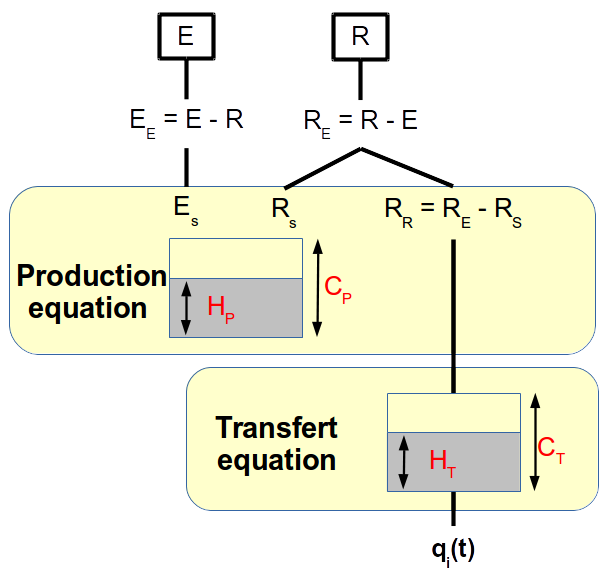
\includegraphics[width=4cm]{modele_grdc.png}
  \end{center}
  
  \caption{Schéma récapitulatif du fonctionnement du modèle GRD.}
  \label{fig:GRD}
\end{figure} 


\subsection{Implémentation de l'algorithme d'assimilation de données 4DVAR}

La fonction coût permettant la résolution d'un problème d'assimilation de données par l'algorithme 4DVar s’écrit sous la forme de l'équation \ref{eq:standardfonctioncoutTikhonov} \citep{gejadze2016discharge} :

\begin{equation}\label{eq:standardfonctioncoutTikhonov}
 J(x,\beta)=\frac{1}{2}||O^{-1/2} (H(x)-y) ||^2 + \frac{\beta}{2}||E^{-1/2}(x-x_b)||^2
\end{equation}

Ou $x$ le vecteur de contrôle contenant les paramètres et états à analyser, $H$ le modèle, $x_b$ le vecteur d'ébauche contenant l'état à priori du système, $O$ la matrice des covariances d'erreurs des observations et $E$ la matrice des covariances des erreurs de l'ébauche. La matrice $E$ étant inconnu, celle-ci est modélisée telle que l'a proposé \citep{gejadze2016discharge}. L'équation \ref{eq:standardfonctioncoutTikhonov} peut-être alors ré-écrite sous la forme suivante :

\begin{equation}\label{eq:fctcoutgrdc}
  J(x)=J_0(x)+ \beta J_{REG}(x)\ \ pour\ \ x>0
\end{equation}

$J_0(x)$ est le coût apporté par les écarts du modèle H(x) au vecteur d'observation $y$ : il s'agit dans notre cas du calcul des résidus entre les débits simulés et observés.\\
$J_{REG}(x)$ est le coût du terme de régularisation et $\beta$ un coefficient à déterminer. Ce terme mesure d'une part l'écart du vecteur de contrôle optimal $x_a$ avec le vecteur d'ébauche $x_b$, et d'autre part la variabilité spatiale des paramètres (contraintes de corrélation). Ce terme doit garantir l'existence d'une solution unique.\\


\subsection{Le cas d'étude : le bassin versant du Gardon d'Anduze}

Ce bassin versant de 540 $km^2$, à Anduze, est situé au cœur des Cévennes (France). Cinq stations de mesures des hauteurs d'eau, associées à leurs courbes de tarage, sont opérationnelles sur ce bassin-versant (figure \ref{fig:BV} et tableau \ref{tab:caracstations}). 

\begin{minipage}{0.5\textwidth}
  \begin{table}[H]
      \caption{Caractéristiques des cinq stations de contrôle.}
      \label{tab:caracstations}
        \begin{center}
          \begin{tabular}{|p{4cm}|p{1.5cm}|p{1cm}|}
          \hline
           Noms des stations  & Codes & Surface ($km^2)$ \\ \hline
           Le Gardon de Mialet à Mialet	& V7124015 & 220\\\hline
           Le Gardon de Mialet à Générargues	& V7124010 & 244\\\hline
           Le Gardon de Saint-Jean à Saint-Jean-du-Gard	& V7135017 & 158\\\hline
           Le Gardon de Saint-Jean à Corbès	& V7135010 & 261\\\hline
           Le Gardon d'Anduze à Anduze	& V7144010 & 541\\\hline
          \end{tabular}
        \end{center}
      \end{table}
\end{minipage}
\hfill
\begin{minipage}{0.45\textwidth}
   
  \begin{figure}[H]
    \begin{center}
      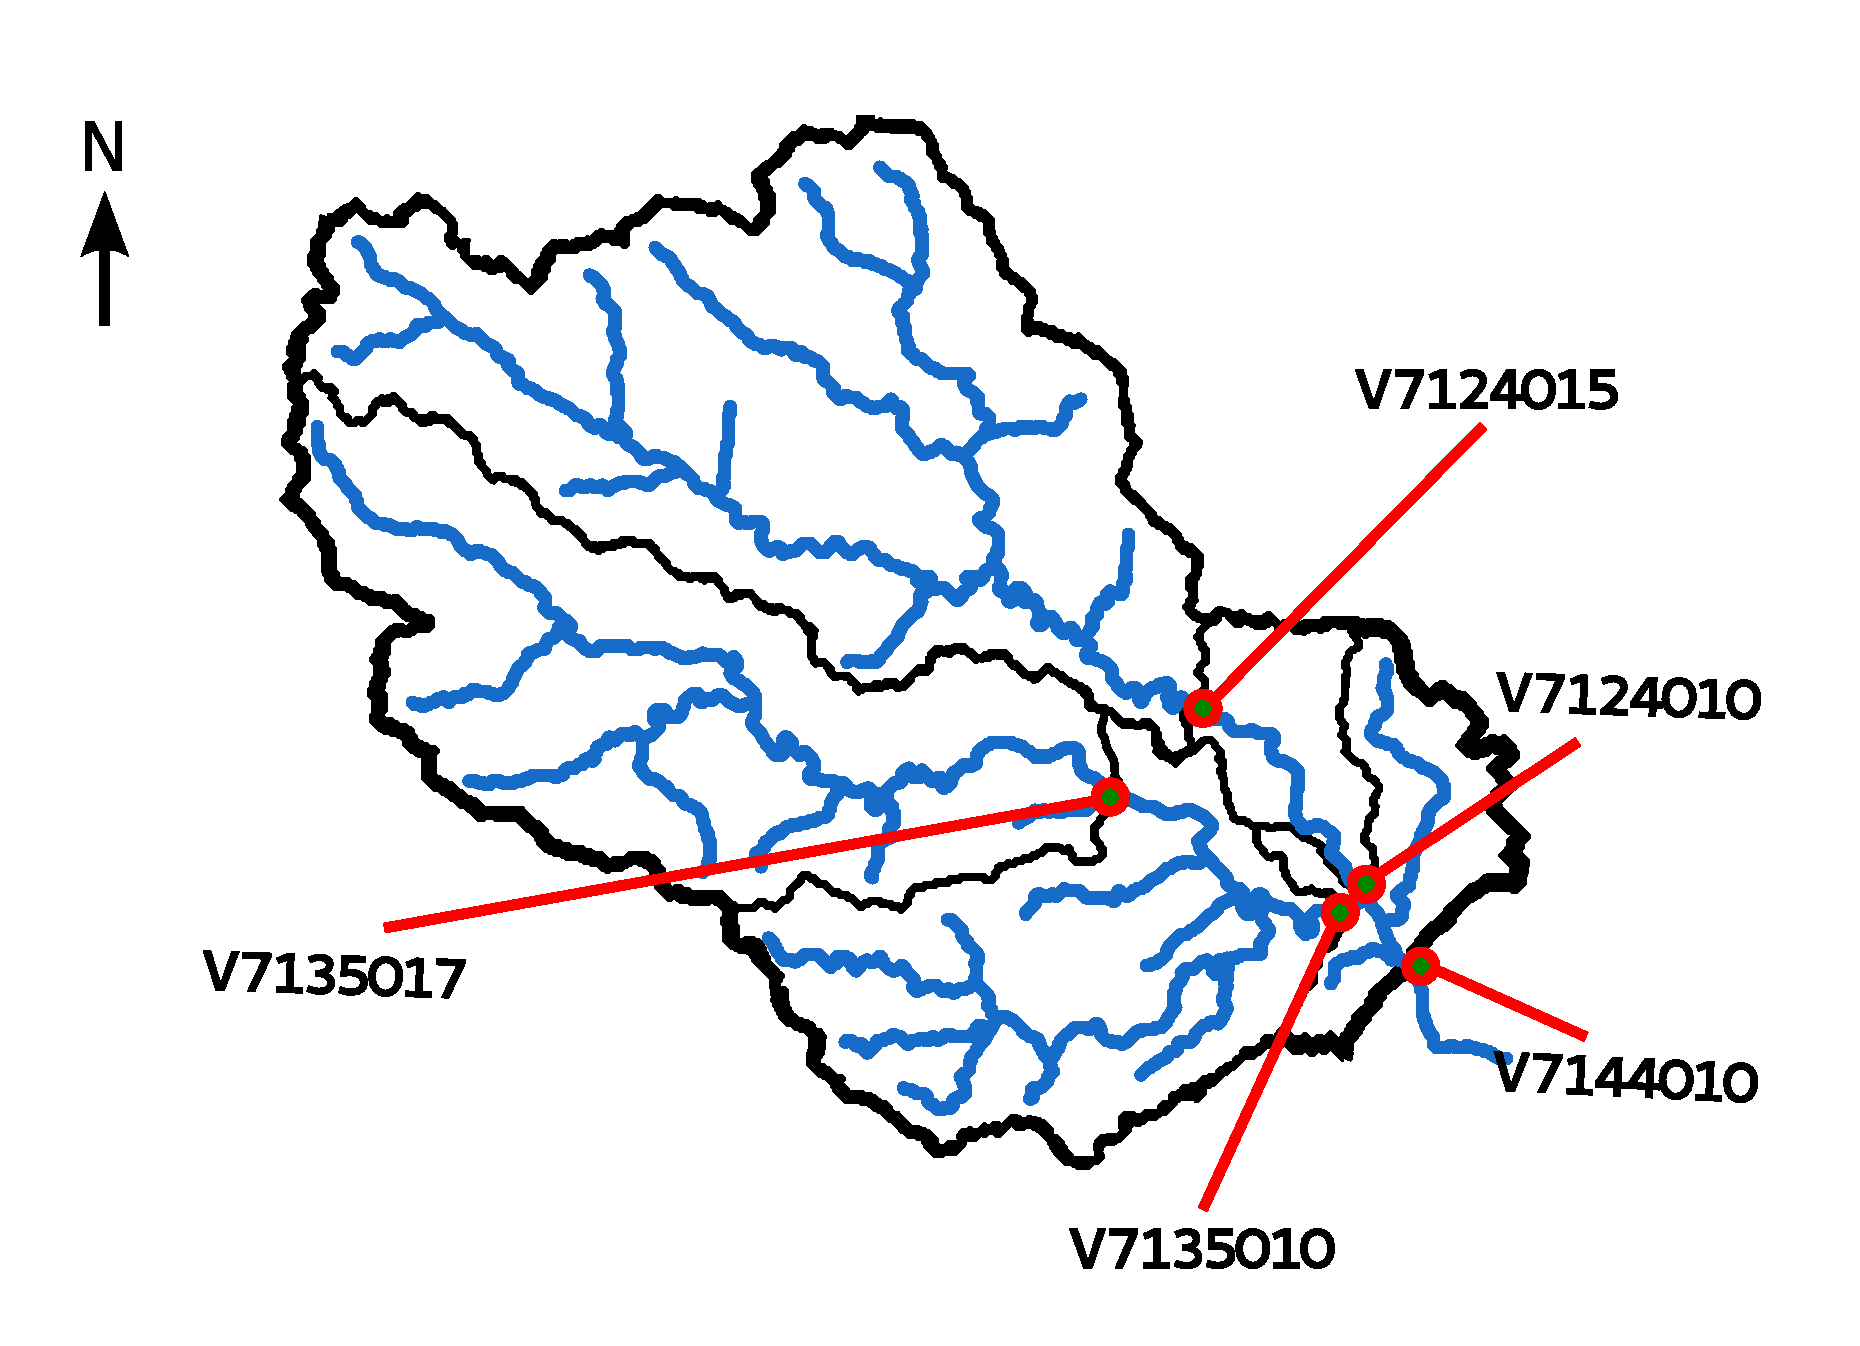
\includegraphics[width=6cm]{Carte_gardon.pdf}
      \caption{Le bassin-versant du Gardon d'Anduze, son réseau hydrographique (bleu) et ses 5 stations de contrôle (V7124015, V7124010, V7135017, V7135010, V7144010).}
      \label{fig:BV}
    \end{center}
  \end{figure}

\end{minipage}
 
  

\section{Conclusions}

L'algorithme d'assimilation variationnelle 4Dvar peut être utilisé pour calibrer les paramètres d'un modèle pluie-débit distribué. Les expériences en calage ont permis de démontrer l’efficacité de cette méthode en menant à d’excellents résultats. Il semble que seule la station de contrôle aval soit suffisante pour calibrer l'ensemble des paramètres du bassin-versant.\\
Cependant, les paramètres trouvés ne peuvent être reliés aux caractéristiques du bassin-versant. Il est notamment nécessaire d'améliorer la modélisation du routage des débits de chaque pixel vers les exutoires, qui dans cette version du modèle manque de sens physique. Ces résultats devront aussi être validés sur un plus grand échantillon de bassins-versants.

\bibliographystyle{plainnat}
\bibliography{biblio}

\end{document} 
